% !Mode:: "TeX:UTF-8"
\documentclass{report}
\usepackage[hyperref, UTF8]{ctex}
\usepackage[dvipsnames]{xcolor}
\usepackage{amsmath}
\usepackage{amssymb}
\usepackage{amsfonts}
\usepackage{listings}
\usepackage{pgfplotstable}
\usepackage{graphicx,float,wrapfig}
\usepackage{pgfplots}
\usepackage{fontspec}
\usepackage{hyperref}
\usepackage{booktabs} % 表格上的不同横线
\usepackage{ifthen}
\usepackage{longtable}
\usepackage[top = 1in, bottom = 1in, left = 1in, right = 1in]{geometry}

% for mac
% \setmonofont[Mapping={}]{Monaco}  %英文引号之类的正常显示,相当于设置英文字体
% \setsansfont{Monaco} %设置英文字体 Monaco, Consolas,  Fantasque Sans Mono

% for windows
\setmonofont[Mapping={}]{Monaco}  %英文引号之类的正常显示,相当于设置英文字体
\setsansfont{Monaco} %设置英文字体 Monaco, Consolas,  Fantasque Sans Mono

\newcommand{\image}[3][3in]{
    \begin{figure}[H]
        \centering\includegraphics[width=#1]{images/#2}
        \caption{#3}
    \end{figure}
}

\newcommand{\miniimage}[3][2.5in] {
    \begin{minipage}[H]{0.4\linewidth}
        \centering\includegraphics[width=#1]{images/#2}
        \caption{#3}
    \end{minipage}
}

\newcommand{\itembf}[1]{\item \textbf{#1}}

\newcommand{\tabletwo}[2] {
    \begin{table}[H] \centering
    \begin{tabular}{ c c }
    \toprule
    \textbf{#1} & \textbf{#2} \\
    \midrule
}

\newcommand{\tabletwoL}[2] {
    \begin{table}[H] \centering
    \begin{tabular}{ l l }
    \toprule
    \textbf{#1} & \textbf{#2} \\
    \midrule
}

\newcommand{\tablethree}[3] {
    \begin{table}[H] \centering
    \begin{tabular}{ c c c }
    \toprule
    \textbf{#1} & \textbf{#2} & \textbf{#3} \\
    \midrule
}

\newcommand{\tablethreeL}[3] {
    \begin{table}[H] \centering
    \begin{tabular}{ l l l }
    \toprule
    \textbf{#1} & \textbf{#2} & \textbf{#3} \\
    \midrule
}

\newcommand{\tablefour}[4] {
    \begin{table}[H] \centering
    \begin{tabular}{ c c c c }
    \toprule
    \textbf{#1} & \textbf{#2} & \textbf{#3} & \textbf{#4} \\
    \midrule
}

\newcommand{\tablefourL}[4] {
    \begin{table}[H] \centering
    \begin{tabular}{ l l l l }
    \toprule
    \textbf{#1} & \textbf{#2} & \textbf{#3} & \textbf{#4} \\
    \midrule
}

\newcommand{\tablefive}[5] {
    \begin{table}[H] \centering
    \begin{tabular}{ c c c c c }
    \toprule
    \textbf{#1} & \textbf{#2} & \textbf{#3} & \textbf{#4} & \textbf{#5} \\
    \midrule
}

\newcommand{\tablefiveL}[5] {
    \begin{table}[H] \centering
    \begin{tabular}{ l l l l l }
    \toprule
    \textbf{#1} & \textbf{#2} & \textbf{#3} & \textbf{#4} & \textbf{#5} \\
    \midrule
}

\newcommand{\tablesix}[6] {
    \begin{table}[H] \centering
    \begin{tabular}{ c c c c c c }
    \toprule
    \textbf{#1} & \textbf{#2} & \textbf{#3} & \textbf{#4} & \textbf{#5} & \textbf{#6} \\
    \midrule
}

\newcommand{\tablesixL}[6] {
    \begin{table}[H] \centering
    \begin{tabular}{ l l l l l p{5cm} }
    \toprule
    \textbf{#1} & \textbf{#2} & \textbf{#3} & \textbf{#4} & \textbf{#5} & \textbf{#6} \\
    \midrule
}

\newcommand{\longtablesixL}[6] {
    \begin{longtable}{ l l l l l p{4.3cm} } 
    \toprule 
    \textbf{#1} & \textbf{#2} & \textbf{#3} & \textbf{#4} & \textbf{#5} & \textbf{#6} \\
    \midrule
}

\newcommand{\tableend} {
    \bottomrule
    \end{tabular}
    \end{table}
}

\newcommand{\longtableend} {
    \bottomrule
    \end{longtable}
}

\newcommand{\chuhao}{\fontsize{42pt}{\baselineskip}\selectfont}
\newcommand{\xiaochuhao}{\fontsize{36pt}{\baselineskip}\selectfont}
\newcommand{\yihao}{\fontsize{28pt}{\baselineskip}\selectfont}
\newcommand{\erhao}{\fontsize{21pt}{\baselineskip}\selectfont}
\newcommand{\xiaoerhao}{\fontsize{18pt}{\baselineskip}\selectfont}
\newcommand{\sanhao}{\fontsize{15.75pt}{\baselineskip}\selectfont}
\newcommand{\sihao}{\fontsize{14pt}{\baselineskip}\selectfont}
\newcommand{\xiaosihao}{\fontsize{12pt}{\baselineskip}\selectfont}
\newcommand{\wuhao}{\fontsize{10.5pt}{\baselineskip}\selectfont}
\newcommand{\xiaowuhao}{\fontsize{9pt}{\baselineskip}\selectfont}
\newcommand{\liuhao}{\fontsize{7.875pt}{\baselineskip}\selectfont}
\newcommand{\shibahao}{\fontsize{18pt}{\baselineskip}\selectfont}
\newcommand{\shisihao}{\fontsize{14pt}{\baselineskip}\selectfont}
\newcommand{\qihao}{\fontsize{5.25pt}{\baselineskip}\selectfont}

\definecolor{mygreen}{rgb}{0,0.6,0}
\definecolor{mygray}{rgb}{0.5,0.5,0.5}
\definecolor{mymauve}{rgb}{0.58,0,0.82}
\lstset{ %
    backgroundcolor=\color{white},   % choose the background color
    basicstyle=\footnotesize\ttfamily,        % size of fonts used for the code
    columns=fullflexible,
    breaklines=true,                 % automatic line breaking only at whitespace
    captionpos=b,                    % sets the caption-position to bottom
    tabsize=4,
    backgroundcolor=\color[RGB]{245,245,244},            % 设定背景颜色
    commentstyle=\color{mygreen},    % comment style
    escapeinside={\%*}{*)},          % if you want to add LaTeX within your code
    keywordstyle=\color{blue},       % keyword style
    stringstyle=\color{mymauve}\ttfamily,     % string literal style
    showstringspaces=false,                % 不显示字符串中的空格
    frame=none,
    rulesepcolor=\color{red!20!green!20!blue!20},
    % identifierstyle=\color{red},
    language=python,
}

% 设置hyperlink的颜色
\newcommand\myshade{85}
\colorlet{mylinkcolor}{violet}
\colorlet{mycitecolor}{YellowOrange}
\colorlet{myurlcolor}{Aquamarine}

\hypersetup{
  linkcolor  = mylinkcolor!\myshade!black,
  citecolor  = mycitecolor!\myshade!black,
  urlcolor   = myurlcolor!\myshade!black,
  colorlinks = true,
}


\title{\yihao{Air Guitar} \\ \erhao{Playing the guitar in the air} \\\erhao{HCI项目总结}}
\date{}
\author{张钰晖 2015011372 185-3888-2881 yuhui-zh15@mails.tsinghua.edu.cn\\
陈齐滨 2015011403 130-0128-2511 chenqibin422@gmail.com\\
周正平 2015011314 189-1196-3301 zhouzp15@mails.tsinghua.edu.cn}
\begin{document}
\maketitle
\clearpage
\tableofcontents
\graphicspath{ {images/} }

\chapter{问题背景}

    \section{为什么要选这个题?}

        \subsection{自然}
        相比平板电脑上有GUI的数字乐器,使用手势识别的系统最大程度地保留了弹奏着与乐器互动\
        的可玩性;同时由于使用了摄像头代替触控屏,使用户的体验更加轻松、自然,活动范围更大。\
        尤其使对于右手,扫弦时不会有触控屏带来的非常影响体验的阻力。

        \subsection{便捷}
        空气吉他相比于传统吉他,有数字乐器一样便于携带、不用调音的优点。

        \subsection{全民}
        尽管本应用使用的是Leap Motion,但事实上在任何有Depth Camera甚至仅RGB Camera\
        系统上,只要部署了手势识别系统,都可以实现这样的吉他。因此在未来大多数人都不需要购买\
        乐器就可体验虚拟乐器,进而帮助发现自己喜欢的乐器。


    \section{什么是吉他?}
    一种食物。就是右手可以把六根弦一口吞下或者一根一根吃。 TODO

    \section{现有的项目如何?}

        \subsection{Virtual Guitar}
        现有的类似项目的一个典型是名为Virtual Guitar的项目。该项目不考虑左手的动作\
        右手也只能点击实现指弹,本质上只是套用了点击功能并在相应位置,放上吉他的弦。该项目\
        有用户手位置的实时反馈来帮助用户操作。在我们对左手选取和弦的实现中借鉴了这个思路,\
        并且研究了是否提供反馈对操作准确度的影响。


\chapter{项目要点}

    \section{项目目标}

        本项目的目标是实现\textbf{吉他扫弦}功能,吉他扫弦可以概括为\textbf{左手和弦,右手扫弦}。

        扫弦是吉他的\textbf{特色}之一,容易上手,结合声乐可以\textbf{弹唱}大部分流行歌曲,对\textbf{精度}要求不太高,同时结合指弹,可以给用户带来完整的用户体验。
        
    \section{左手和弦}

        为了能扫出不同和弦,我们需要左手来选择和弦。在普通吉他中,左手用手指在按下六根弦中的\
        不同离散的位置(称为“品”),也可以不按。这样不同的按法,就能让右手扫弦时产生不同的和弦声音。

        \image[6in]{f}{左手和弦}

        为了解决左手和弦问题,我们提出了以下几个算法。

        \subsection{九宫格算法}

        将和弦抽象成一个个按钮,均匀的分布在空间的9个点上,利用左手食指点击动作选择和弦以代替整个手的和弦动作。

        优点是操作方便,容易上手,实现简单。缺点是可用和弦数量有限。

        \subsection{1-近邻算法}

        左手每个手指分别获取位置后,判断每个手指是否按到弦。

        优点是实现简单,适合指弹。缺点是无法利用和弦固定位置的信息。

        \subsection{条件概率算法}

        参考《ATK: Enabling Ten-Finger Freehand Typing in Air Based on 3D Hand Tracking Data》论文,主要是采用条件期望公式,利用某个和弦下,输入的先验概率分布。

        $$P(C|I)=\frac{P(C) \times P(I|C)}{P(I)}\propto P(C)\times P(I|C)$$

        公式中I为input(输入),C为chord(和弦)。

        优点是能充分利用和弦信息,把每个和弦看做word,能大大提高准确率。缺点是实现较复杂,需要事先得到$P(I|C)$。

        \subsection{神经网络算法}

        收集左手数据,利用左手数据的信息训练出一个神经网络(MLP),通过训练好的神经网络进行分类。

        优点是学科交叉,神经网络算法准确率一般较高。缺点是需要收集大量数据,且容易过拟合开发者的弹奏习惯。

        \subsection{增强算法}

        \begin{enumerate}
            \item{加入手指信息}:一个和弦中按的弦与手指对应,可以加入输入端点位置对应的手指信息提高准确率。
            \item{预测和弦进行}:一般乐曲和弦的进行都是有规律的,如经典旋律C-G-Am-Em-F-G-C,可以加入乐曲进行信息提高准确率。
            \item{加入反馈信息}:软件方面视觉上给出合适的反馈,从而使用户可以在弹奏中学习适应。
        \end{enumerate}

        \subsection{最终算法}

        左手和弦时手掌朝向身体内侧,由于Leap Motion精度问题,在桌面上放置Leap Motion时无法捕捉到左手手指的信息,并且由于空间中没有标“品”的位置,非常容易弹错,因此1-近邻算法、条件概率算法、神经网络算法均无法使用。

        最终我们选择九宫格算法来实现左手和弦的选择,我们选择C调的常用和弦以九宫格的形式呈现给用户(可以通过软件轻易的进行修改),对应到空间中就是一个虚拟的九宫格,左手用点击来选择和弦。

        由于Leap Motion SDK中提供的KeyTap检测效果较差,我们自己实现了左手KeyTap检测算法,并采用了增强算法中的加入反馈信息方式,通过手对应位置和选择确认的界面反馈提升用户体验。

     \section{右手扫弦}

        在吉他弹奏过程中,右手按照音乐的节拍扫动没有被禁用的弦,在左手的和弦下,便会发出一段精美的乐音。

        \image[6in]{e}{右手扫弦}

        相比左手和弦算法,右手扫弦算法实现相对较为简单,我们提出以下算法。

        \subsection{空间固定算法}

        六根弦在空间中位置固定,利用右手的位置、速度、走向、高度等信息做分类,弹奏响应的弦。

        \subsection{问题}

        右手扫弦最大的问题是连续同方向扫弦问题,由于吉他右手节奏型中经常存在连续向相同方向扫弦的问题,因此必须解决这个问题。

        \image[6in]{strumming}{连续同方向扫弦问题}

        一种解决方案是,通过软件控制,做成音乐游戏的形式,提前录入曲谱,只响应节拍上的动作。

        另一种解决方案是,根据右手高度信息加以判断,同时结合图形界面给用户反馈,从而使用户可以在弹奏中学习如何控制深度。

        我们最终采用了第二种方案。
       



\chapter{实现细节}

    \section{整体框架?}

        \subsection{MVP}
        采用MVP模式,后端提供处理LM帧后得到的吉他信息接口,前端界面使用这些接口获取和弦设置、\
        右手位置等信息。

        \subsection{Leap Motion摄像头数据的获取}
        为了提高开发效率,我们选择了Python sdk,运行在本地,处理帧并且提供吉他的数据;\

        \subsection{用户界面}
        用户界面写的是网页前端,可以较快地实现不错的界面。\

        同时,这样可以把前后端分离开来,就算后端不是基于Leap Motion的,\
        只要接口一致,我们的用户界面可以通用。

        另一个这样考虑原因是可扩展性,如果我们需要用到多个Leap Motion(虽然最后没有做),\
        因为需要用到多台主机(python sdk不支持一台主机连多个LM),使用web传递数据将非常方便。

        最终界面请参考Chapter 3。


    \section{音乐库?}
    使用了FluidSynth软音源,包含各种MIDI中典型乐器的音色,使用mingus.midi.fluidsynth\
    提供的接口使用。来模拟一个音的产生,音高范围为两位的16进制码表示,即0~127,其中60为中央C,
    如果预先选择了乐器,那么就能播放这个乐器弹这个音的声音。

    需要注意的是,不同于钢琴,由于吉他上不同位置有相同的音,并且音色有细微区别,但是用我们比较简陋\
    的MIDI不能区分这两种,好在对听感影响很小,最终还是很接近真实吉他。

    \section{前后端通信}
    使用了短轮询,这是由于Leap Motion的异步机制与WebSocket的异步机制不能很优雅地兼容,\
    导致后端无法向前端主动推送数据来反应用户双手的变化。只能前端轮询数据,虽然效率有所降低,\
    但使用过程中并没有发觉到卡顿。


\chapter{项目展示}

    \section{用户界面}
    制作提供了\textbf{拟物化主题}和\textbf{扁平化主题}两套主题。

    \image[6in]{g}{拟物化主题}

    \image[6in]{h}{扁平化主题}

    两套主题制作都较为精美细致,保留了吉他本身的特点。

    \section{和弦选择界面}

    当用户左手进行和弦选择时,红色框将在九宫格上滑动,来实时地反馈弹奏者手指地位置,当弹奏者\
    找到所需和弦时,降低左手位置超过一阈值就会触发和弦的设置。

    从交互角度来看,可以认为这是通过反馈来减少误选;
    从吉他弹奏角度来看,也可以理解成需要把弦按下力度达到一定程度才能达到效果,而不是轻碰就可以,\
    类似实际弹奏的逻辑。

    \image[6in]{i}{和弦选择界面(拟物化主题)}

    \image[6in]{j}{和弦选择界面(扁平化主题)}

    \section{触弦振动界面}
    右手的操作我们也提供了反馈。可以看到界面上展示了吉他以及六根弦,当弹奏者右手触到相应位置时,\
    发出和弦对应弦的乐音,对应弦将给出合适的振动效果,使其看起来更加逼真。

    \image[6in]{k}{弦振动界面(拟物化主题)}

    \image[6in]{l}{弦振动界面(扁平化主题)}

    \section{后台运行}
    后端的Python脚本会持续运行处理并呈现数据,输出日志便于调试。

    \image[6in]{m}{后端输出}



\chapter{用户实验与数据分析}

    \section{Goal}
    为了研究项目中的(A左手九宫格确认反馈/B新手准确率学习曲线),我们设计了如下实验并进行了分析。

    \section{Participants}
        \paragraph{Number}
        n个
        \paragraph{Gender}
        19-21岁 男???
        \paragraph{Familiarity with the task}
        都是选/未选修 HCI 课程、会/不会弹吉他

    \section{Apparatus}
        \paragraph{Hardware}
        Leap Motion version几来着 TODO

        \paragraph{Software}
        用户界面统一都使用了暖色系主题。

        \paragraph{Environment}
        室温、坐姿、日光照明

    \section{Procedure}

    \section{Result(准确率如何?大概多久能学会?用户满意度?)}

    \section{Analysis(拿到了什么数据?简单分析发现了什么?或者验证了什么?)}


\chapter{总结与展望}

    \section{项目总结}
    % 实现了什么,有什么优点?
    % TODO:maybe not professional, please modify if necessary
    % TODO: need some data
    本次实验实现了一个基于Leap Motion的吉他扫弦应用,其主要成果包括如下几个方面:

        \subsection{右手扫弦交互}
        在AirGuitar中,右手负责扫弦。

            \paragraph{实现方式} 我们通过模拟真实吉他扫弦的交互方式,在用户右手的惯用位置水平虚拟构造了6根弦,符合吉他弹奏者的使用习惯。
            当用户的右手在Leap Motion的指定高度之上扫过,对应位置处的弦便会接连被触发,从而发出一串动人的旋律。

            \paragraph{实现效果} 经过测试,我们发现,右手扫弦交互可以在绝大多数情况下精准识别用户扫过的弦。

            大部分用户可以在3分钟左右的训练时间内达到90\%左右的扫弦正确率,而在经过1小时左右的熟悉过程之后则可达到100\%。
            并且,用户仅需简单的学习过程,便可以掌握高度的控制方法,从而使得扫弦与否的误操作率达到正常弹奏可以忍受的级别。

        \subsection{左手选择和弦交互}
        在AirGuitar中,左手负责选择和弦。

            \paragraph{实现方式} 我们通过将真实吉他选择和弦的方式加以简化,将其接口抽象为简洁的九宫格形式,同时在其中置入最常见的和弦,兼顾了简洁性和可用性。
            当用户的左手水平移动到指定的坐标,并以手指点击时,对应位置处的和弦便会被选择,从而改变用户扫弦时发出的音调。% TODO:音调?响度?音色?

            \paragraph{实现效果} 经过测试,我们发现,在为界面加入反馈确认机制之后,用户可以在较短的时间内学会使用左手选择和弦。

            大部分用户可以在3分钟左右的训练时间内达到65\%左右的和弦选择准确率,而在经过1小时的熟悉过程之后,则可达到90\%-100\%。

        \subsection{用户界面}
        在AirGuitar中,用户界面为用户提供可视化的交互方式,并提供反馈机制、视觉线索等。

            \paragraph{实现方式} 用户界面使用HTML5+CSS+JS实现,使用浏览器渲染,轻量且可跨平台。

            其主界面分为2大部分:扫弦区域(对应右手)与和弦选择九宫格(对应左手)。

            \begin{enumerate}
                \itembf{反馈机制}:界面为右手扫弦和左手选择和弦均提供了反馈机制。当用户右手扫弦时,被扫过的弦会播放一段震动动画;
                当用户左手选择和弦时,被选和弦会被高亮为不同颜色。

                \itembf{视觉线索}:界面提供了完善的视觉线索,UI动态将用户左手在九宫格中的当前位置渲染高亮。
                同时,用户按下选择和弦时,UI会将对应位置高亮为不同颜色。
            \end{enumerate}

            \paragraph{实现效果} 经过测试,我们发现,简洁美观的界面极大地降低了用户的学习成本,并提升了使用体验。

            用户在反馈机制与视觉线索的引导下,也能显著地降低误操作率,从而提高演奏的流畅度。这一点笔者对比开发初期和后期的调试效率可谓深有体会。

    \section{瓶颈以及解决方案}

        \subsection{识别范围}

            \paragraph{瓶颈分析}
            轻松的弹奏操作需要给用户足够大的动作幅度空间,然而Leap Motion并不能提供这么大的识别范围\
            若右手离开识别范围,则再次进入时会有不能忍受的较大延时。若减少右手作用幅度,扫弦非常流畅且容易控制,\
            达到预期目标。

            \paragraph{解决方案}
            一个可能的解决方案是增加手到Leap Motion的高度,由于Leap Motion识别范围为锥体,因此\
            这样可以增加平面上的活动范围。但是手举太高容易使弹奏者疲劳,也不符合吉他弹奏的感觉。

        \subsection{双手干扰}
            \paragraph{瓶颈分析}
            开发过程中我们注意到,单独对左右手的调试都可以达到我们想要实现的目标,比如左手选一个和弦\
            序列,右手扫出想要的pattern等。但是一旦到了两者结合起来,不仅双手能活动的范围变小,\
            双手的坐标准确度也没有只有一只手的时候高。

            \paragraph{解决方案}
            可以尝试用两个Leap Motion,由于一开始调研的时候也想到可能双手会比较挤的情形,\
            在写用户界面的时候,我们的数据交换是基于TCP的,这样的方式可以方便地应用到\
            多个Leap Motion的数据分工获取与交换,便于后续工作(如果有的话)。


\chapter{开发周期}


    \section{合作方法}

        \subsection{开发环境}
        % Leap Motion官方Python2 SDK, 具体的环境说明以及配置方法见Git仓库的README。
        % TODO:The repo is private... although TA may never visit it.
        项目使用Leap Motion官方Python2 SDK进行开发,代码托管在GitHub仓库上\footnote{https://github.com/yuhui-zh15/AirGuitar}。

            \paragraph{后端开发环境} 后端开发环境主要指使用Leap Motion Python SDK实现的事件处理后台。

            % TODO:although failed to make it work on Windows T^T
            以下所有工具均可在Windows、Mac OS、Linux中的任意一个平台上运行,实现了跨平台开发。

            \tablethreeL{工具}{版本号}{简要说明}
                Leap Motion Python2 SDK & 2.3.1 & 用于感知用户双手的运动并转化为事件帧 \\
                fluidsynth & 依具体平台而不同 & 音乐库,包含各种MIDI中典型乐器的音色 \\
                mingus & 0.5.1 & Python音乐库模块,用于编程调用 \\
                flask & 0.12.2 & Python Web框架,用于和前端通信 \\
                flask-cors & 3.0.3 & 用于在flask框架上实现跨域资源共享(CORS) \\
            \tableend

            \paragraph{前端开发环境} 前端开发环境主要指基于HTML+CSS+JavaScript开发的用户界面。

            \tablethreeL{工具}{版本号}{简要说明}
                jQuery & 1.11.0 & 用于简化JavaScript代码结构 \\
            \tableend

            \paragraph{文档工具} 文档工具用于为项目构建清晰的接口说明文档。
            \tablethreeL{工具}{版本号}{简要说明}
                sphinx & 1.6.5 & 文档生成工具 \\
                sphinx-rtd-theme & 0.2.4 & 文档主题库 \\
            \tableend

        \subsection{设计模式}
            \paragraph{观察者模式(Observer)}
            ChordHandler, StrummingHandler分别处理Leap motion到来的帧,分开左手与右手的处理,并且不用修改主程序。

            \paragraph{组合(Aggregation)} 一个吉他模拟器Guitar实例将提供set\_chord, play\_string方法,使\
            处理输入数据后可以方便地改变吉他的状态。

    \section{迭代开发}

        \subsection{开发计划}
        以下给出AirGuitar的迭代开发计划:

            \paragraph{Sprint 1} 环境配置、初步实现左右手交互功能。
            \begin{enumerate}
                \itembf{音乐库}:选择并配置Python跨平台音乐库。
                \itembf{右手扫弦初步实现}:初步实现右手扫动时发出乐音的功能。
                \itembf{左手选择和弦初步实现}:初步实现九宫格式选择和弦功能,并留好接口以备扩展。
            \end{enumerate}

            \paragraph{Sprint 2} 功能完善、UI制作。
            \begin{enumerate}
                \itembf{右手扫弦功能完善}:通过高度限制,增强右手扫弦防误触功能。
                \itembf{左手选择和弦完善}:增加左手和弦识别功能。
                \itembf{UI}:基于Web框架实现UI,为后台准备接口。
            \end{enumerate}

            \paragraph{Sprint 3} 连接前后端、精度提升。
            \begin{enumerate}
                \itembf{前后端通信}:通过轮询方式实现后台和前端UI的数据通信。
                \itembf{左手选择和弦精度提升}:通过在UI增加反馈机制、视觉线索等,提高左手选择和弦的精度。
            \end{enumerate}

            \paragraph{Sprint 4} 用户实验、完成文档。
            \begin{enumerate}
                \itembf{用户实验}:收集学习时间、操作准确度等数据。
                \itembf{开发文档}:进行项目总结,完成文档。
            \end{enumerate}

        \subsection{版本控制}
        使用Git作为版本控制和分支管理的工具,任务分配通过GitHub上的Issue功能开展。

        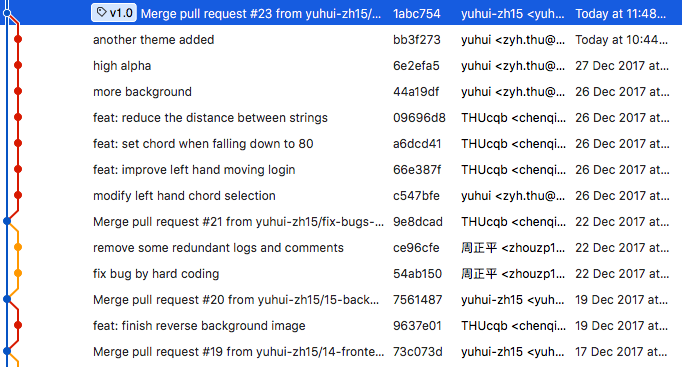
\includegraphics[width=\textwidth]{git}

        \subsection{项目管理}
        Merge Request组员都会收到并且互相进行Code Review,使我们代码质量较高、\
        开发进度也一直较快,在阶段展示的时候完成度就已经非常高。

        由于设备只有一台,故大多数时候其实并不能并行开发。




% \section{算法实现}

% \subsubsection{BasicRNNCell}

%     \paragraph{算法原理} BasicRNNCell为最基础的一类Cell,从输入到输出,实现的仅为最简单的线性变换,并加以激活,无门机制控制记忆的写入与遗忘:
%     $$h_t = \tanh([h_{t-1}, x_t] \cdot W + b)$$
%     \image[4in]{BasicRNNCell}{BasicRNNCell}

%     \paragraph{实现方法} 实现时,只需模拟上述公式即可:

    % \begin{enumerate}
    %     \itembf{词向量导入}: 在\texttt{main.py}中导入预训练的词向量;
    %     \itembf{模型搭建}: 在\texttt{model.py}中实现\texttt{placeholder}等,搭建基于RNN的神经网络;
    %     \itembf{基本单元}: 在\texttt{cell.py}中实现BasicRNNCell, GRUCell, BasicLSTMCell等基础单元;
    %     \itembf{模型可视化}: 在\texttt{main.py}中加入TensorBoard可视化代码。
    % \end{enumerate}

    % \begin{lstlisting}
    % for vocab in vocab_list:
    %     if vocab in embed_dict:
    %         embed.append(embed_dict[vocab])
    %     else:
    %         embed.append([0.0] * FLAGS.embed_units)
    % \end{lstlisting}

    % \tablethreeL{变量}{形状}{含义}
    %     $x_t$ & $[batch\_size \times embed\_units]$ & 当前时刻的输入 \\
    %     \midrule
    %     $z_t$ & $[batch\_size \times num\_units]$ & update门,候选状态对新状态的影响 \\
    %     $r_t$ & $[batch\_size \times num\_units]$ & reset门,旧状态对候选状态的影响 \\
    %     \midrule
    %     $W_z, b_z$ & $[(embed\_units + num\_units) \times num\_units]$, $[num\_units]$ & update门的变换矩阵、偏置 \\
    %     $W_r, b_r$ & $[(embed\_units + num\_units) \times num\_units]$, $[num\_units]$ & reset门的变换矩阵、偏置 \\
    %     $W, b$ & $[(embed\_units + num\_units) \times num\_units]$, $[num\_units]$ & 从旧状态到候选状态的变换矩阵、偏置 \\
    %     \midrule
    %     $\tilde{h_t}$ & $[batch\_size \times num\_units]$ & 候选状态 \\
    %     $h_t$ & $[batch\_size \times num\_units]$ & 产生的新状态 \\
    % \tableend

    % \image[6in]{loss_gru}{GRUCell loss-epoch曲线}

% \begin{thebibliography}{9}
%     \bibitem{GRUPaper} http://arxiv.org/abs/1406.1078
%     \bibitem{LSTMPaper} http://arxiv.org/abs/1409.2329
%     \bibitem{RNNTutorial} https://zhuanlan.zhihu.com/p/28196873
%     \bibitem{LSTMTutorial} http://colah.github.io/posts/2015-08-Understanding-LSTMs/
%     \bibitem{GRUTutorial} http://blog.csdn.net/meanme/article/details/48845793
%     \bibitem{BiLSTMTutorial} http://blog.csdn.net/wuzqChom/article/details/75453327
% \end{thebibliography}

\end{document}
